\documentclass[12pt]{article}


\usepackage{amssymb}
\usepackage{amsmath}
\usepackage{fullpage}
\usepackage{epsfig}
\usepackage{epstopdf, xcolor, hyperref}
\everymath{\displaystyle}

\newif\ifans

\anstrue

\begin{document}

\begin{center}
\underline{\LARGE{Work}}
\end{center}

\bigskip

\noindent SUGGESTED REFERENCE MATERIAL:

\bigskip

\noindent As you work through the problems listed below, you should reference Chapter 6.6 of the recommended textbook (or the equivalent chapter in your alternative textbook/online resource) and your lecture notes.

\bigskip

\noindent EXPECTED SKILLS:

\begin{itemize}

\item Be able to use integration to compute the work done by a variable force in moving an object along a straight path from $x=a$ to $x=b$.  Specifically, be able to solve Spring Problems, Lifting Problems, \& Pumping Problems.

\end{itemize}

\section*{Conceptual Problems}

\begin{enumerate}

\item A variable force $F(x)$ is applied in the positive $x$ direction, as shown in the graph below.

\begin{center}
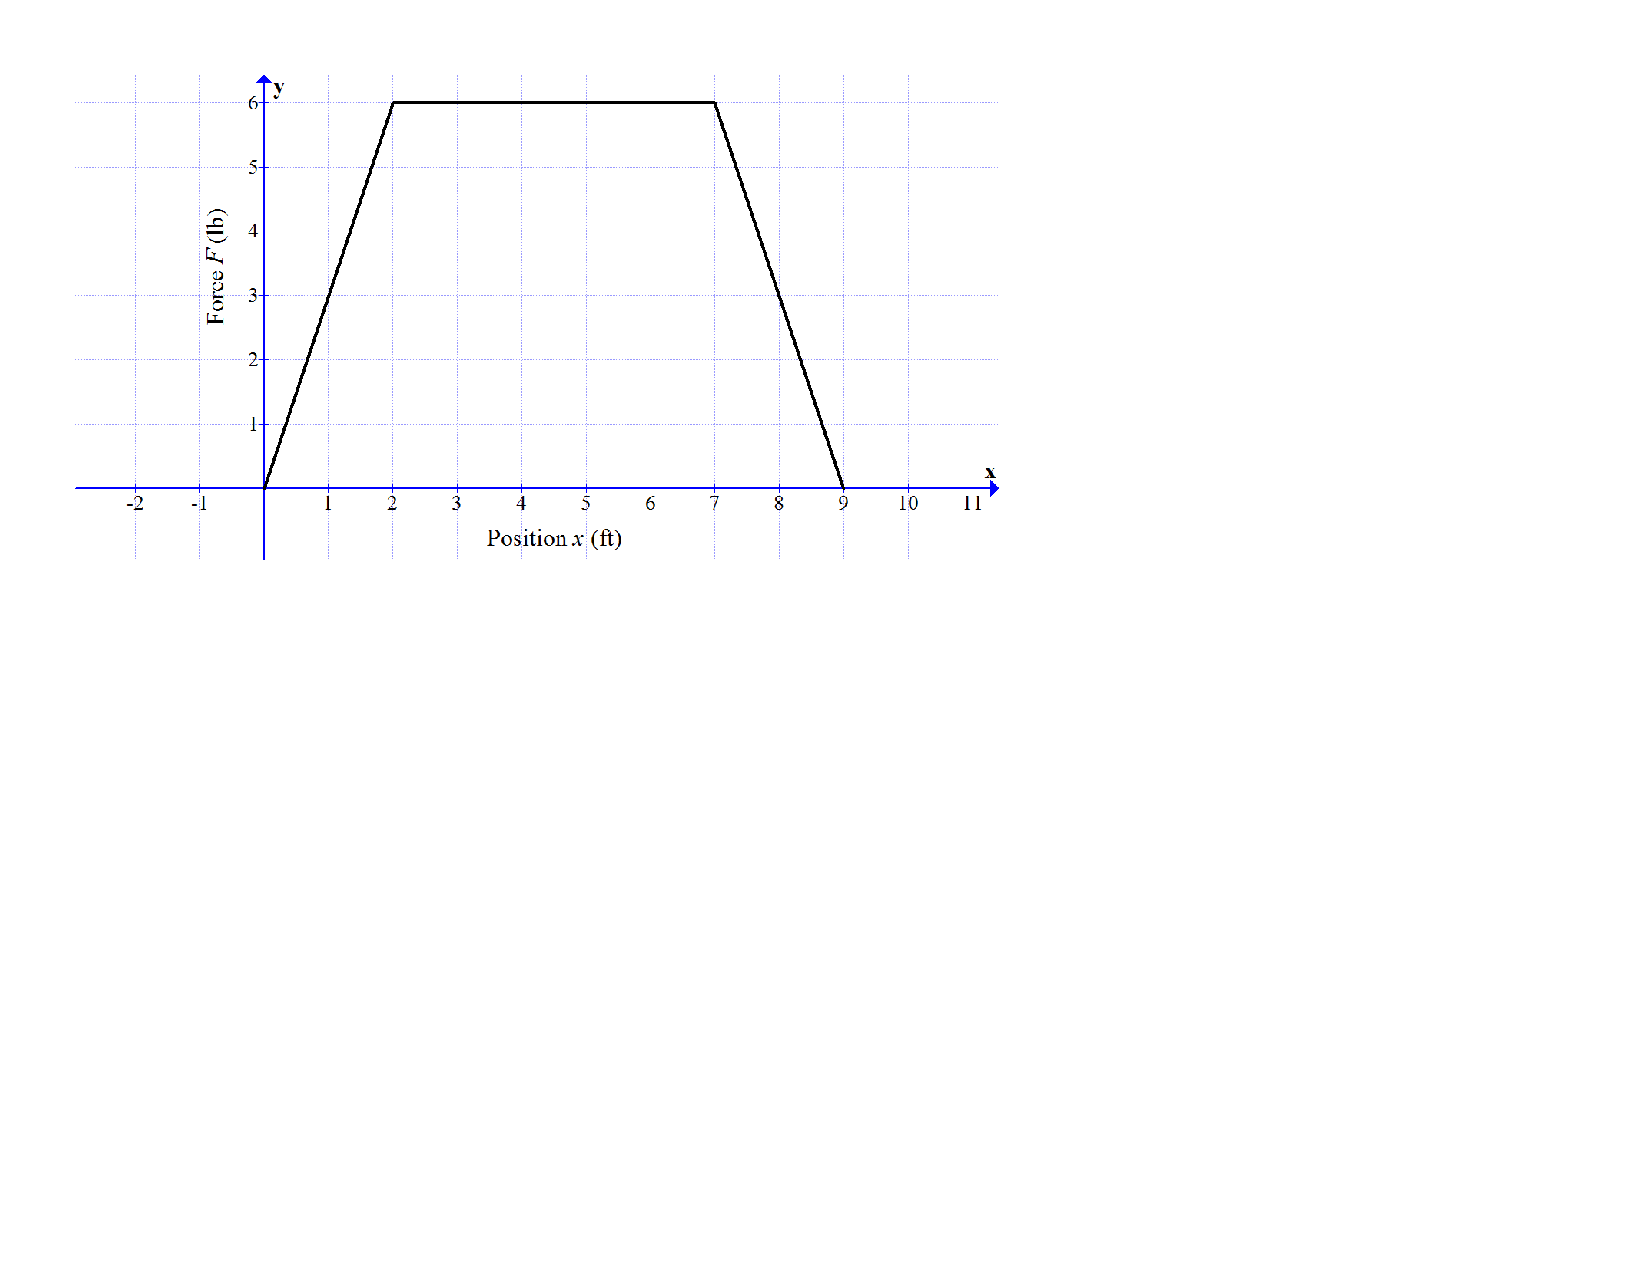
\includegraphics[scale=0.6]{graph1.pdf}
\end{center}

Find the work done by the force in moving a particle from $x=0$ to $x=9$.

\ifans{\fbox{42 ft$\cdot$lb}} \fi

\end{enumerate}

\section*{Spring Problems}

\begin{enumerate}
\setcounter{enumi}{1}

\item A force of 20 lb is required to hold a spring stretched 5 in beyond its natural length.  How much work is done in stretching the spring from its natural length to 7 in beyond its natural length?

\ifans{\fbox{$98 \text{ in}\cdot\text{lb}=\frac{49}{6} \text{ ft}\cdot\text{lb}$ }} \fi

\item A spring has a natural length of 2 ft.  A body of 10 lb hanging on the spring stretches it to a total length of 2.4 ft.

\begin{enumerate}

\item Find the spring constant (in pounds per foot).

\ifans{\fbox{$F(x)=kx$, where $k=25$}} \fi

\item  How far beyond its natural length would a body of 50 lb stretch the spring?

\ifans{\fbox{The spring will stretch 2 ft beyond its natural length to a total length of 4 ft.}} \fi

\item How much work is required to stretch the spring from its natural length to a length of 3 ft?

\ifans{\fbox{$\frac{25}{2} \text{ ft}\cdot\text{lb}$; Detailed Solution: \textcolor{blue}{\href{http://www.math.drexel.edu/classes/Calculus/resources/Math122HW/Solutions/122_10_Work_03.pdf}{Here}}}} \fi

\end{enumerate}

\item If the work required to stretch a spring 1 foot beyond its natural length is 15 ft$\cdot$lb, how much work is needed to stretch it 8 inches beyond its natural length? (Hint: 1 foot = 12 inches)

\ifans{\fbox{$\frac{20}{3} \text{ ft}\cdot\text{lb}$}} \fi

\end{enumerate}

\section*{Lifting Problems}

\begin{enumerate}
\setcounter{enumi}{4}
\item A cable that weighs 3 lb/ft is used to lift 1,000 lb of iron ore up a mineshapft which is 450 ft deep.  Find the work done.

\ifans{\fbox{753,750 ft$\cdot$lb}} \fi

\item A 5 lb bucket containing 10 lb of water is hanging at the end of a 30 ft rope which weighs $\frac{1}{2}$ lb/ft.  The other end of the rope is attached to a pulley.  Assume that the rope is wound onto the pulley at a rate of 3 ft/s causing the bucket to be lifted. Find the work done in winding the rope onto the pulley.

\ifans{\fbox{675 ft$\cdot$lb; Detailed Solution: \textcolor{blue}{\href{http://www.math.drexel.edu/classes/Calculus/resources/Math122HW/Solutions/122_10_Work_06_07.pdf}{Here}}}} \fi

\item Repeat problem 6 adding the assumption that water leaks out of the bucket at a rate of $\frac{1}{4}$ lb/s.

\ifans{\fbox{$\frac{1275}{2}$ ft$\cdot$lb; Detailed Solution: \textcolor{blue}{\href{http://www.math.drexel.edu/classes/Calculus/resources/Math122HW/Solutions/122_10_Work_06_07.pdf}{Here}}}} \fi

\item A bag of sand originally weighing 144 lb is lifted at a constant rate.  As it rises, sand also leaks out at a constant rate.  At the instant when the bag has been lifted to a height of 18 feet, exactly half of the original amount of sand remains.  (Neglect the weight of the bag and the lifting equipment.)

\begin{enumerate}

\item Describe the weight of the sand as a function of $x$, where $x$ is the height of the bag above the ground.

\ifans{\fbox{$w(x)=144-4x$}} \fi

\item Calculate the work done in lifting the sand to the height of 18 ft from the ground.

\ifans{\fbox{1944 ft$\cdot$lb}} \fi

\end{enumerate}

\end{enumerate}

\section*{Pumping Problems}

\begin{enumerate}
\setcounter{enumi}{8}

\item A circular swimming pool has a diameter of 10 meters.  The sides are 4 meters high.  And, the depth of the water is 3.5 meters.  How much work is required to pump all of the water over the side?  Recall that water weighs 9810 N/m$^3$.

\ifans{\fbox{$6.067 \times 10^6$ J}} \fi

\item At Charlie's Chocolate Factory, a tank in the shape of an inverted right circular cone has a height of 10 meters and a radius (at the top) of 6 meters is filled with chocolate pudding to a height of 2 meters.  In order to sterilize the tank, the factory needs to empty the tank.  Find the work required to empty the tank by pumping the chocolate pudding through a hole in the top of the tank. Note: the weight-density of chocolate pudding is 12,178 N/m$^3$.

\ifans{\fbox{$\frac{2,484,312}{25}\pi$ J}} \fi

\item The trough pictured below is 15 feet long and 4 feet wide at the top.  The ends of the trough are isosceles triangles with a height of 3 feet.  
\begin{center}
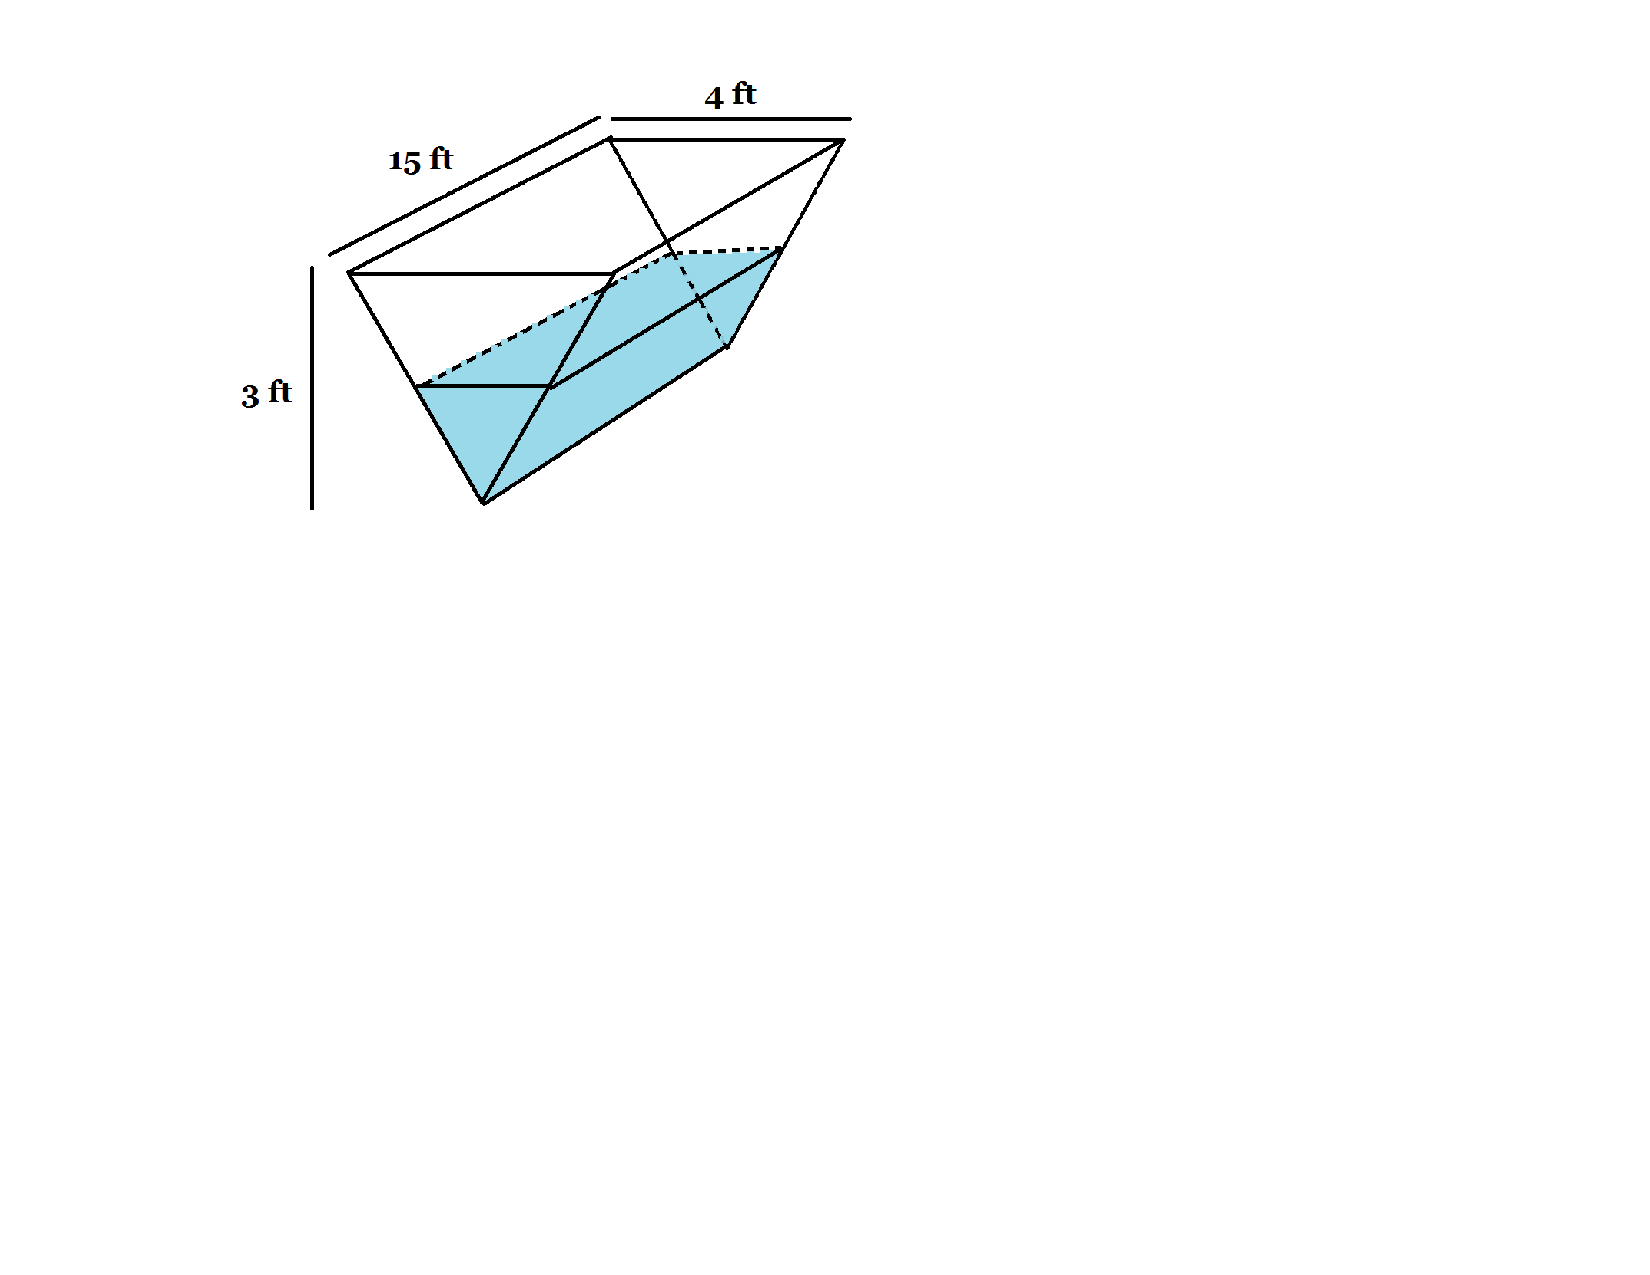
\includegraphics[scale=0.6]{trough.pdf}
\end{center}
If the trough is filled to a height of 1 foot with water, find the work required to pump all of the water over the side?  Recall that water weighs 62.4 lb/ft$^3$.

\ifans{\fbox{1,456 ft$\cdot$lb}} \fi

\newpage

\item The tank shown below is half full of oil which has a weight-density of 9016 N/m$^3$.  
\begin{center}
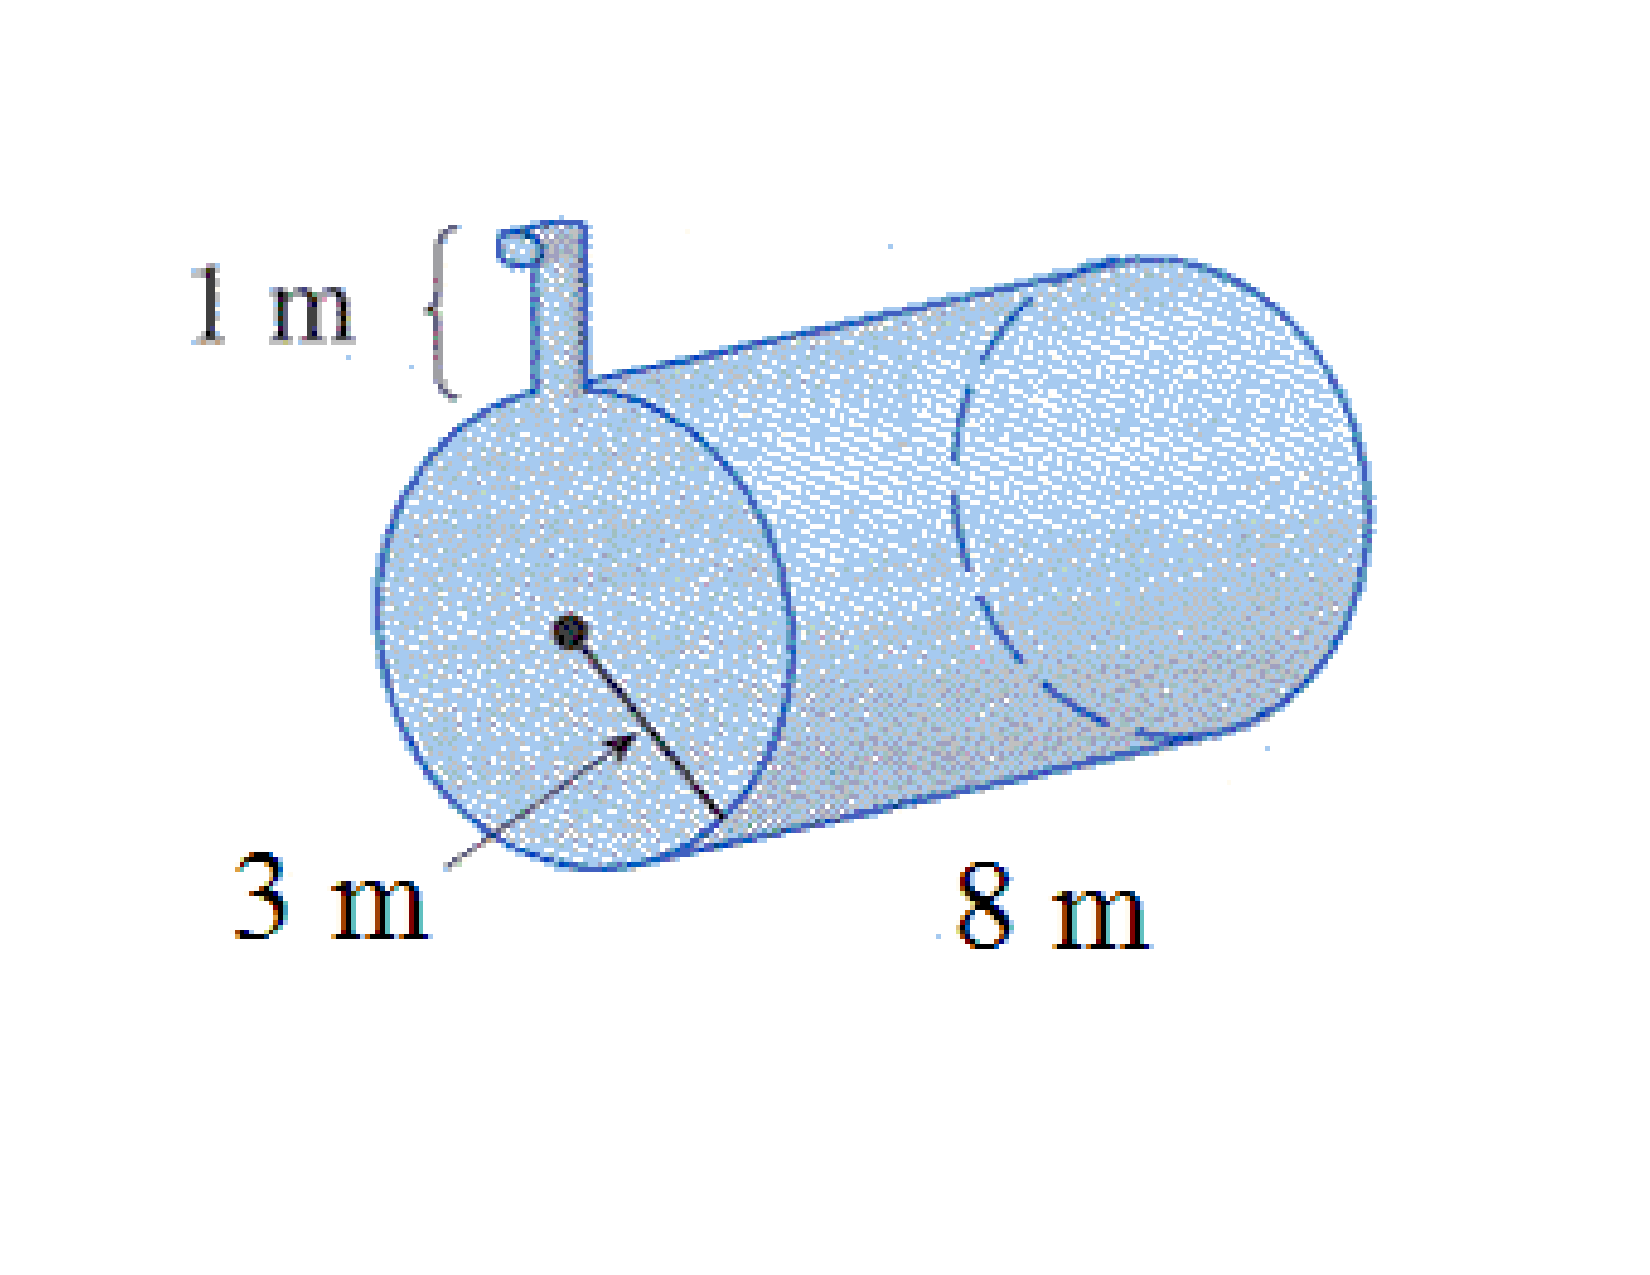
\includegraphics[scale=0.3]{tank.pdf}
\end{center}
Let $x=0$ correspond to the bottom of the tank.  Set up an integral which represents the work (in joules) required to pump the oil out of the outlet at the top which is one meter above the top of the tank.  {\bf Do not evaluate your integral.}

\ifans{\fbox{$W=\int_0^3 9016 \cdot 8 \cdot 2 \cdot \sqrt{9-(3-x)^2} \cdot (7-x) \,dx= 144,256 \int_0^3 (7-x)\sqrt{6x-x^2}\,dx$ J}} \fi

\end{enumerate}

\end{document}